\section{Materials and Methods}

\subsection{Study 1: Evaluateion bias and variance of cross-validation}

This study investigated the interplay between sample size and various performance estimators and their collective impact on bias and variance during model validation. It is hypothesized that increasing the sample size will reduce both bias and variance. Additionally, it is expected that the validation variance will increase with the number of folds in the CV, while simultaneously reducing bias. Since K-fold CV employs a fraction (i.e., $K-1$ folds) of the data for training, it may provide a pessimistic estimate of model performance. This study seeks to measure the degree of performance underestimation for each cross-validation estimator, which include in-sample, 2-fold, 5-fold, 10-fold, and LOOCV.

The design of the simulation assesses performance estimators, including K-fold CV with K set to 2, 5, and 10, as well as LOOCV where K equals the sample size N, and the "In-Sample" evaluation, which assesses model performance on the same dataset used for training, potentially leading to an overly optimistic bias. To gauge model performance, three metrics are employed: RMSE (Eq. ~\ref{eq_rmse}), r (Eq. ~\ref{eq_r}), and $R^2$ (Eq. ~\ref{eq_R2}). The validation model is a multivariate linear regression with ten input features and one output target, all drawn from a standard normal distribution $\mathcal{N}(0, 1)$, implying no expected linear relationship between inputs and the target, with an expected correlation r of zero. The sample sizes N are varied among 50, 100, and 500 to explore the dynamics between sample size and performance estimators. Each configuration is repeated across 1000 iterations to assess the distribution of bias and variance.

For each iteration, the dataset $\mathcal{D}={(X, Y)}$ was sampled as per the simulation’s premise. In the case of K-fold CV, the dataset $\mathcal{D}$ was partitioned into K folds in which each fold is $\mathcal{D}_k={(X_k, Y_k)}$. For the “In-Sample” approach, partitioning does not occur. The linear model f is trained on the training set $\mathcal{D}_\text{-k}$ (denoted as $f_{\mathcal{D}_{\text{-k}}}$) to estimate regression coefficients $\beta$, which then predicts the target variable ${\hat{Y}}_k$ from the test set $\mathcal{D}_k$. The procedure of K-fold CV can be expressed as:


\begin{equation} \label{eq_kfoldcv}
    \begin{split}
	\text{Training: } \quad Y_{\text{-k}} &= f_{\mathcal{D}_{\text{-k}}}(X_{\text{-k}})+\epsilon \\
    &= X_{\text{-k}} \beta + \epsilon \\
    \text{Testing: } \quad \hat{Y}_k &= f_{\mathcal{D}_{\text{-k}}}(X_k) \\
    &=X_k \beta \quad \quad \quad k=1,2,\ldots,K 
    \end{split}
\end{equation}

For the “In-Sample” performance estimator, predictions were made without splitting, as:

\begin{equation} \label{eq_insample}
    \begin{split}
    	\text{Training: } \quad Y &= f_\mathcal{D}(X) \\ &= X\beta + \epsilon \\
        \text{Testing: } \quad \hat{Y} &= f_\mathcal{D}(X) \\ &=X \beta
    \end{split}
\end{equation}

Where:
\begin{itemize}
  \item \( X \) denotes the input regressors sampled from a standard normal distribution \( \mathcal{N}(0, 1) \) with dimensions \( N \times 10 \).
  \item \( Y \) denotes the target variable sampled from a standard normal distribution \( \mathcal{N}(0, 1) \) with dimensions \( N \times 1 \).
  \item \( X_\text{-k} \) and \( Y_\text{-k} \) are the input regressors and target variable in the training set \( \mathcal{D}_\text{-k} \).
  \item \( X_k \) denotes the input regressors in the test set \( \mathcal{D}_k \).
  \item \( \hat{Y}_k \) denotes the predicted target variable in the test set \( \mathcal{D}_k \).
  \item \( \beta \) denotes the estimated regression coefficient with dimensions \( 10 \times 1 \).
  \item \( \epsilon \) denotes the error term assumed to be normally distributed.
\end{itemize}

Estimated performance $\mathbb{E}[\hat{g}(f_\mathcal{D})]$ was derived by averaging the performance metrics across all K folds as per Eq. ~\ref{eq_g_exp}. The bias and variance of the evaluation were calculated using Eqs. ~\ref{eq_bias} and ~\ref{eq_var}, respectively. To approximate true model performance $G(f_\mathcal{D})$, a hundred unseen datasets $\mathcal{D}^\ast$ were generated identically to $\mathcal{D}$, and the performance $G(f_\mathcal{D})$ was estimated by averaging the performance metrics across all $\mathcal{D}^\ast$. The detailed steps to compute evaluation bias and variance are provided in the supplementary materials.

\subsection{Study 2: Model Selection in Cross-Validation}

The objective of this simulation study is to examine the effect of improper model selection implementation on validation bias. The focus will be on the model selection procedures of feature selection and hyperparameter tuning. The study hypothesizes that utilizing the test set inappropriately during any model selection stage will lead to a significant overestimation of model performance. This study simulated a regression task using an SVR model, which utilized various kernel functions to project a subset of features, X, to predict a target variable, Y. Both X and Y are drawn from a normal distribution $\mathcal{N}(0, 1)$ to establish a baseline null correlation (performance r=0) for assessing validation bias. This study set the sample size and number of features at 100 and 1000, respectively. Feature selection is executed by choosing the top 50 features that correlate most strongly with Y. For hyperparameter tuning, four kernel functions were evaluated: linear, polynomial, radial basis function, and sigmoid.
\begin{figure}[h]
    \centering
    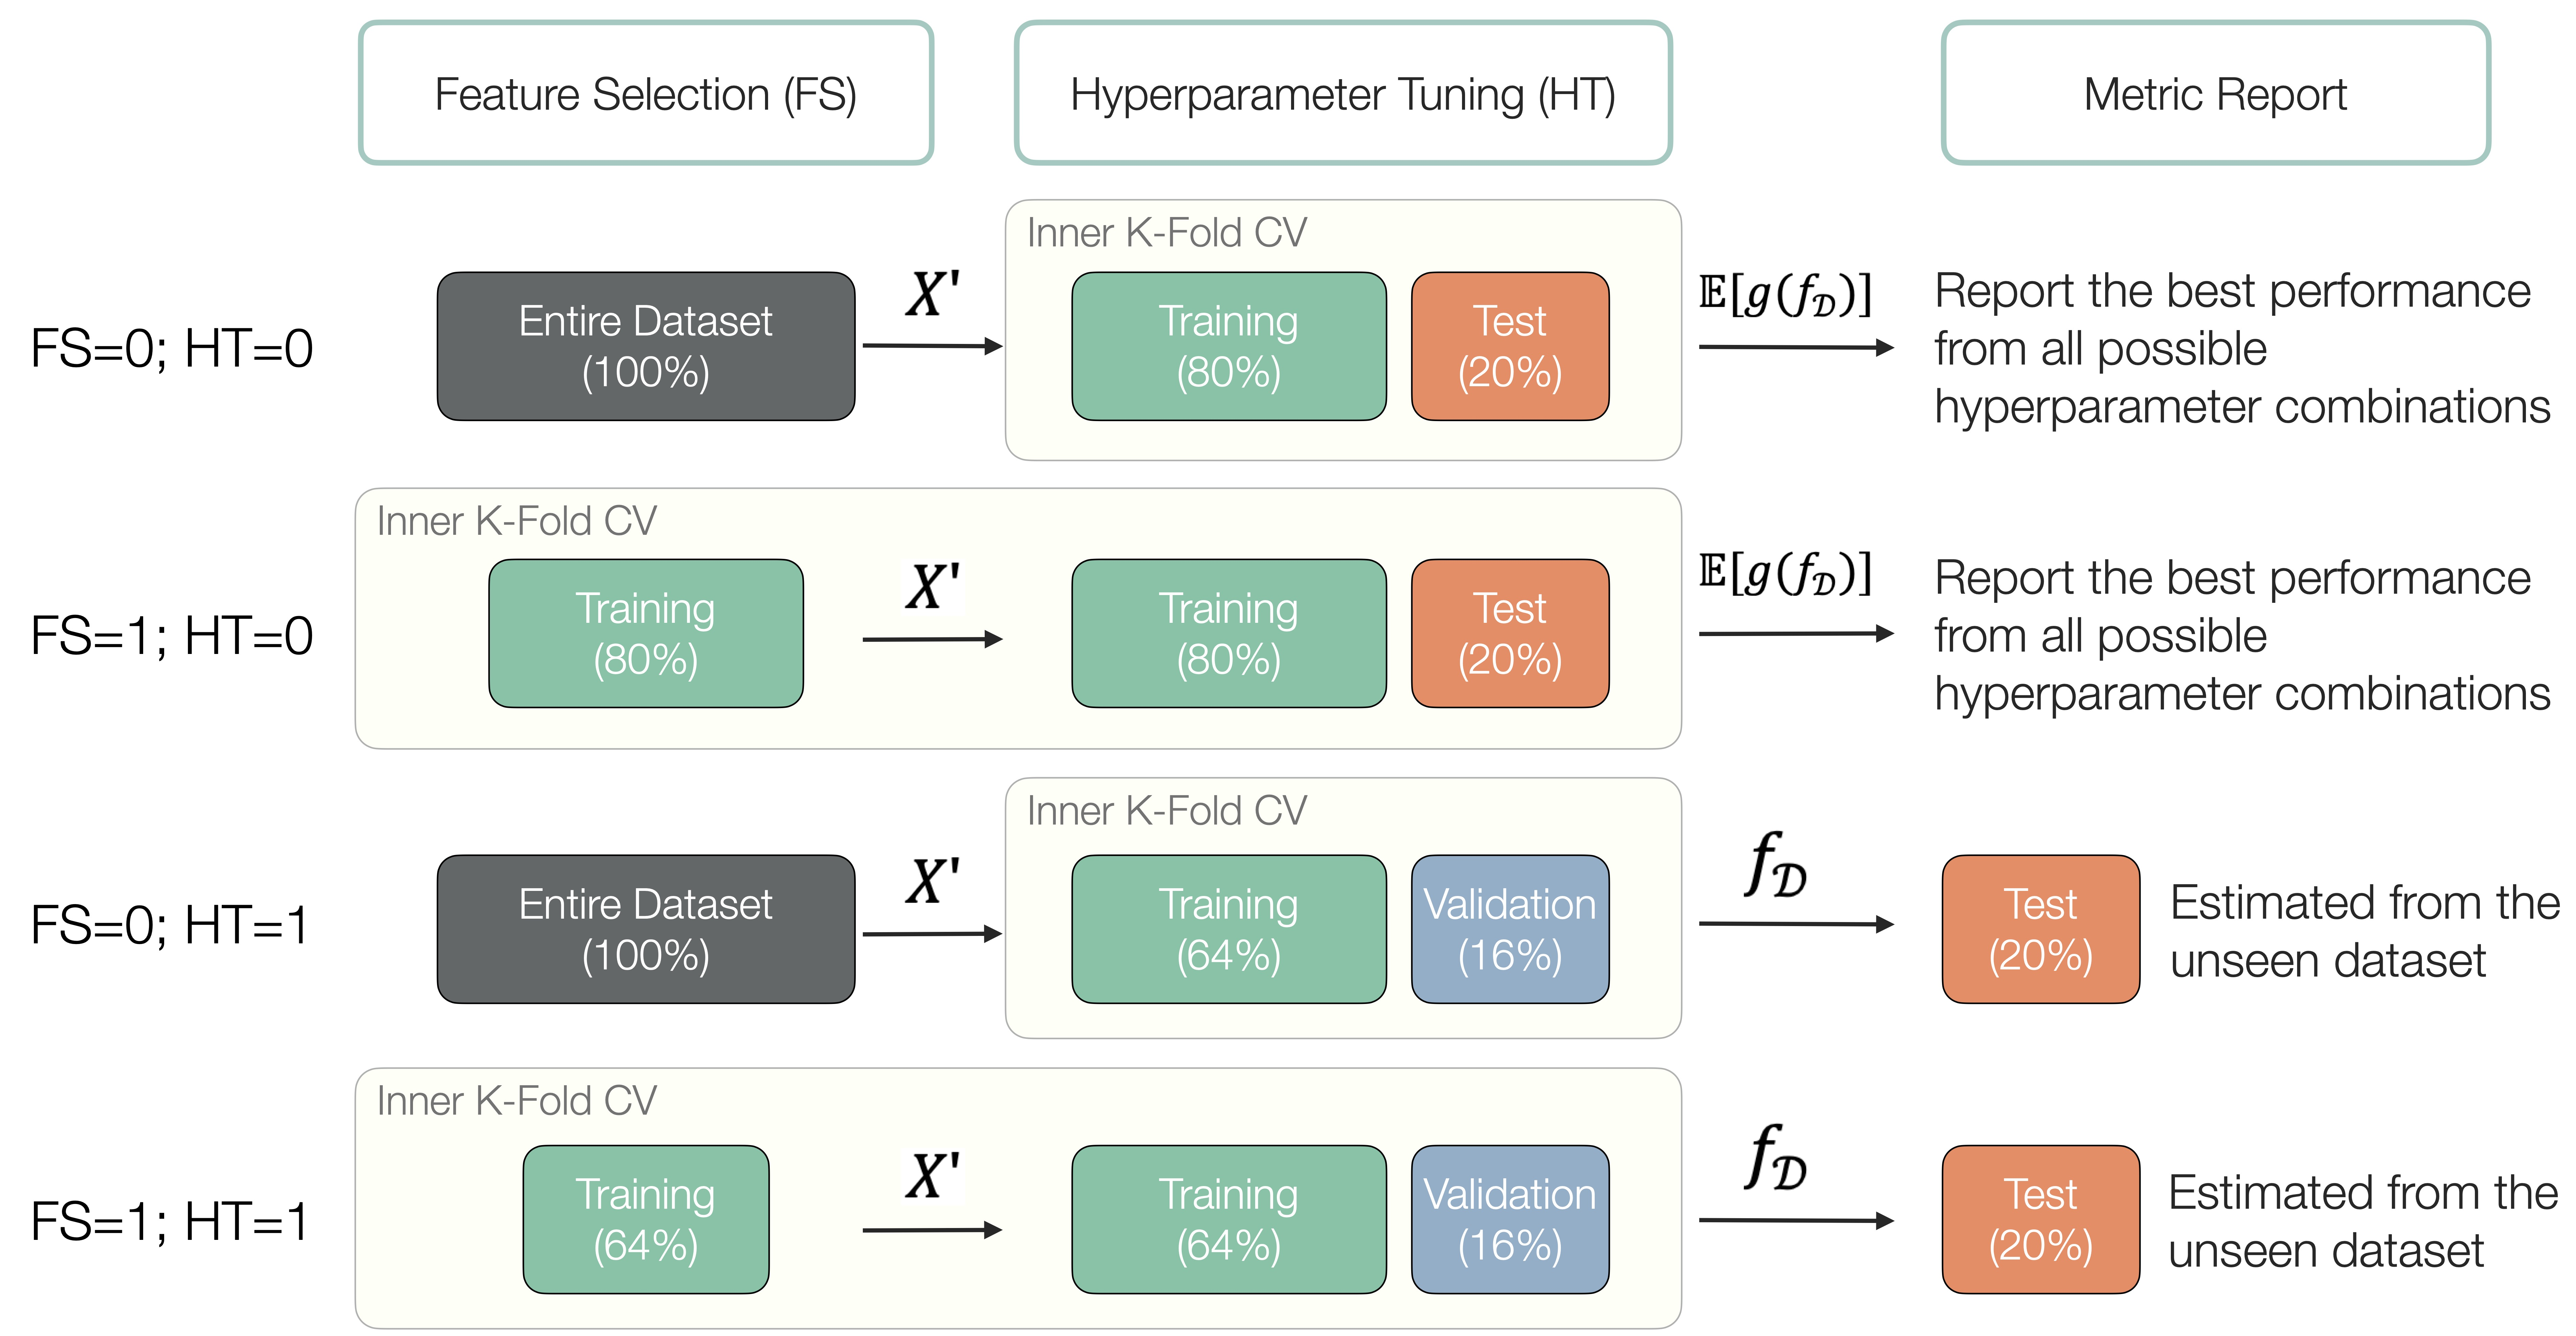
\includegraphics[width=1\textwidth]{fig_s2_schemes.jpg}
    \caption{Workflow diagram illustrating four cross-validation strategies of feature selection (FS) and hyperparameter tuning (HT), where 0 denotes incorrect implementation and 1 indicates correct practice. $X'$ is the selected feature subset, $\mathbb{E}[\hat{g}(f_\mathcal{D})]$ is the expected generalization performance, $f_\mathcal{D}$ is the model trained on the training set without being revealed to the test set.}
    \label{fig:s2_schemes}
\end{figure}

This study introduces notations FS for feature selection and HT for hyperparameter tuning, assigning a binary indicator (0 or 1) to denote incorrect (0) or correct (1) implementation of model selection. This yields four possible combinations of model selection strategies: “FS=0; HT=0”, “FS=0; HT=1”, “FS=1; HT=0”, “FS=1; HT=1” (Figure 7). When FS=0, feature selection precedes cross-validation splitting. If FS=1, feature selection occurs within each fold of the training set during cross-validation. With hyperparameter tuning, a correct implementation (HT=1) involves splitting the dataset into training (64\%), validation (16\%), and test (20\%) sets. The model is trained and tuned using the training and validation sets, respectively, while the test set is reserved for a single evaluation of model performance. Conversely, with HT=0, only training (80\%) and test (20\%) sets are used, risking validation bias as the test set informs both training and performance reporting. A 5-fold cross-validation approach was deployed for all strategies.
Validation bias is measured as the discrepancy between the model selection-influenced performance estimate and the expected generalization performance (r=0), using the Pearson correlation coefficient between predicted and observed values. Over 1000 sampling iterations, the study assesses the distribution of validation bias. A t-test will determine whether the validation bias significantly deviates from zero.

\subsection{Study 3: Block Effects in Cross-Validation}

